\documentclass[11pt,a4paper]{article}

\usepackage[utf8]{inputenc}
\usepackage[T5,T1]{fontenc}
\usepackage{lmodern}
\usepackage{microtype}
\usepackage[margin=1in]{geometry}
\usepackage{amsmath,amssymb}
\usepackage{graphicx}
\usepackage{booktabs}
\usepackage{tabularx}
\usepackage{array}
\usepackage[table]{xcolor}
\usepackage{caption}
\usepackage[section]{placeins}
\usepackage{enumitem}
\usepackage{tikz}
\usetikzlibrary{positioning,fit,arrows.meta,calc}
\usepackage[round,authoryear]{natbib}
\usepackage{xurl}
\usepackage[hidelinks]{hyperref}

\captionsetup{font=small,labelfont=bf}
\setlist{itemsep=2pt,topsep=4pt}
\newcolumntype{Y}{>{\raggedright\arraybackslash}X}
\newcolumntype{P}[1]{>{\raggedright\arraybackslash}p{#1}}
\definecolor{preai}{HTML}{2A78D6}
\definecolor{withai}{HTML}{EB6834}
\definecolor{boxline}{HTML}{8A8984}
% Vietnamese needs the T5 encoding for its stacked diacritics.
\newcommand{\viet}[1]{{\fontencoding{T5}\selectfont #1}}

\title{Miteiru: Designing an Open-Source Subtitle-Immersion Player for Japanese, Mandarin, Cantonese and Vietnamese, Before and With AI Coding Assistants}
\author{Hocky Yudhiono\\[2pt]\small Independent researcher, Hong Kong SAR\\\small\texttt{its@hocky.id}}
\date{8 October 2026}

\begin{document}
\maketitle

\begin{abstract}
Miteiru is an open-source desktop video player for learning Japanese, Mandarin, Cantonese and Vietnamese from the subtitles of real video. It segments each subtitle line into words, shows a reading over every word (furigana, pinyin, Jyutping) and a short gloss under it, and opens a dictionary entry when the learner clicks. Everything runs offline on bundled dictionaries; large language models are an optional layer that never touches the subtitle pipeline. This paper describes its design and architecture, and gives the rationale for twelve design decisions traced to the commits and issues where they were made. It argues that Cantonese needs a language mode of its own, not a Mandarin variant: in a screen of 22 YouTube videos found by Cantonese searches whose uploaders wrote Chinese subtitles, 15 were written in Standard Written Chinese and 6 in written Cantonese, so the words on screen often differ from the words spoken. Miteiru was built in two eras: 497 commits over 32 months written without AI coding assistants (December 2022 to August 2025), then 136 commits over 12 months written with them. In the second era the code grew from 9.7k to 33.6k lines and the test suite from nothing to 33 files, while the median commit grew from 13 to 89 changed lines. The paper reports these measurements, the system's measured limits (Japanese long-vowel readings, Vietnamese segmentation), and its use: 3,983 release downloads and 117 GitHub stars, with no telemetry.
\end{abstract}

\noindent\textbf{Keywords:} language learning; subtitles; interactive captions; furigana; Jyutping; Cantonese; written Cantonese; AI-assisted software development

\section{Introduction}

Watching video in the language one is learning is popular advice, in the spirit of learning from comprehensible input \citep{krashen1985input}, and with target-language subtitles a well-supported one: subtitles in the spoken language help listeners learn to perceive a foreign accent, while subtitles in their own language get in the way \citep{mitterer2009foreign}, and captioned video helps listening comprehension and vocabulary \citep{monteroperez2013captioned,vanderplank2016captioned}. The difficulty is the vocabulary. Television needs about 3,000 word families for 95\% coverage of its words and about 7,000 for 98\% \citep{webb2009vocabulary}, far beyond a beginner, and in Japanese and Chinese an unknown word cannot even be sounded out, because the script does not spell its pronunciation.

Interactive subtitles answer this by making every word a lookup. \citet{kovacs2014smart} showed that learners of Chinese who could hover over subtitle words for definitions could afterwards define more than twice as many new words as with dual subtitles, with no loss in comprehension or enjoyment. Browser extensions such as Language Reactor \citep{languagereactor} and asbplayer \citep{asbplayer}, and pop-up dictionaries such as Yomitan \citep{yomitan}, bring the idea to streaming sites and web pages.

Miteiru (\emph{miteiru}, ``watching'' in Japanese) is a desktop player in this family \citep{miteiru}. It plays local files and YouTube videos with any subtitle file, and for four languages it segments each line into words, puts a reading above each word and a short gloss below it, colours words by how well the learner knows them, and opens a dictionary entry on click (Figure~\ref{fig:teaser}). It began in December 2022 as a Japanese player, added Cantonese a year later and Mandarin a month after that, and Vietnamese in 2025.

This paper is a systems paper with a short first-person account. Its contributions are:
\begin{enumerate}
  \item \textbf{A system} (Sections~\ref{sec:walkthrough}--\ref{sec:languages}): an open-source, offline subtitle-immersion player whose per-language pipelines share one rendering and lookup layer, with measured examples of where each pipeline succeeds and fails.
  \item \textbf{A design rationale} (Section~\ref{sec:decisions}): twelve decisions, each with the alternative it rejected and the commit or issue where it was made.
  \item \textbf{An argument that Cantonese is not a Mandarin setting} (Section~\ref{sec:cantonese}), with a small screen of YouTube subtitles showing that most Cantonese videos are subtitled in Standard Written Chinese, so a learner often reads different words from the ones they hear.
  \item \textbf{A longitudinal account of building it before and with AI coding assistants} (Section~\ref{sec:history}): 633 commits over 45 months, split at the month the author started using them.
\end{enumerate}
The source, the screenshots' inputs and every measurement's data are public (Section~\ref{sec:availability}).

\begin{figure}[t]
  \centering
  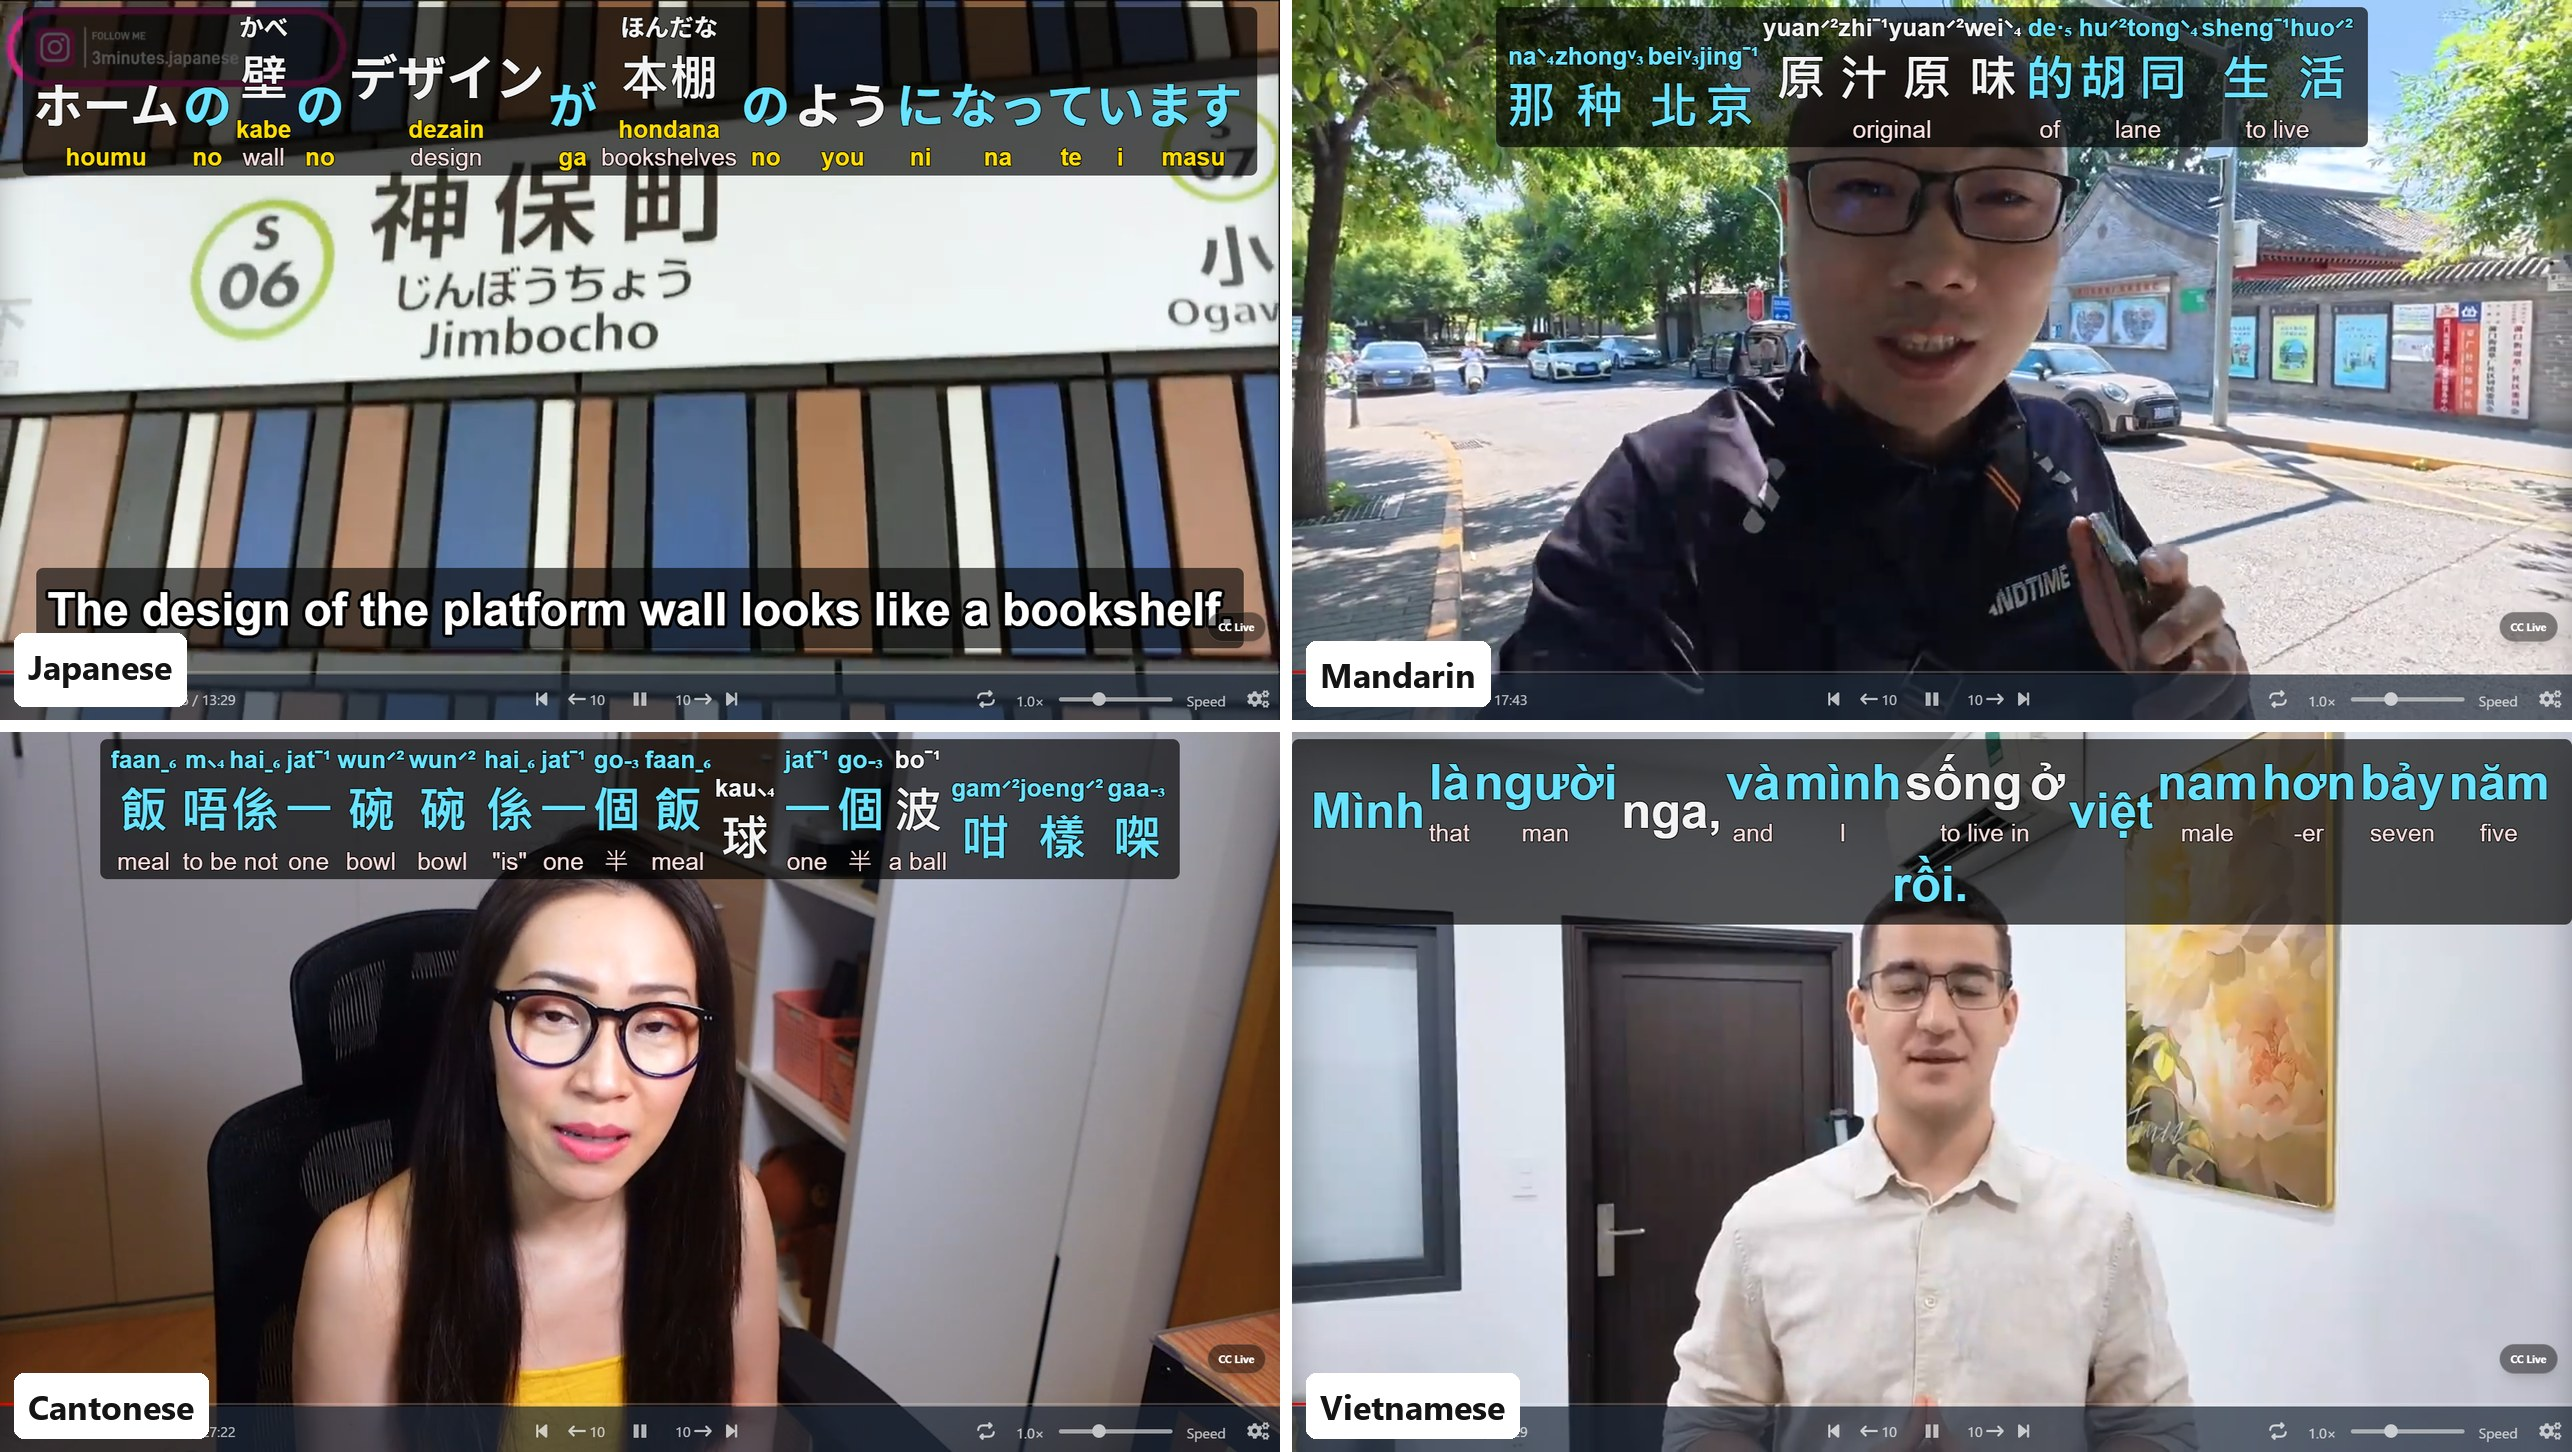
\includegraphics[width=\linewidth]{figures/fig_teaser.jpg}
  \caption{Miteiru 7.5.2 on one line in each language, each from a video whose uploader subtitled the speech in its own language. The primary track (top) is segmented, with readings above and glosses below; colour marks learning state (white: new; cyan: frequent in this video, Section~\ref{sec:display}). Japanese: furigana, romaji and an English secondary track. Mandarin and Cantonese: pinyin and Jyutping with contour tone marks (Figure~\ref{fig:tones}). Vietnamese: glosses only, and two segmentation errors discussed in Section~\ref{sec:vietnamese}. Video frames: see Appendix~\ref{app:sources}.}
  \label{fig:teaser}
\end{figure}

\section{Background and related work}
\label{sec:background}

\paragraph{Subtitles and vocabulary.}
Subtitle research distinguishes captions (same-language subtitles), translated subtitles and dual subtitles. Same-language subtitles help perceptual learning of foreign speech \citep{mitterer2009foreign} and, across studies, listening comprehension and vocabulary \citep{monteroperez2013captioned}. Dual subtitles trade form for meaning: in an eye-tracking study, bilingual subtitles beat captions for recognising word meanings but were worse for recognising word forms \citep{wang2022incidental}, and a study of the Netflix extension that became Language Reactor found dual subtitles helped vocabulary and gave the best listening comprehension \citep{dizon2021netflix}. Miteiru supports both: a primary track in the target language that is analysed, and an optional secondary track, usually a translation, shown as plain text.

\paragraph{Reading aids.}
For learners of Chinese, how the romanisation is shown matters. Pinyin presented at the same time as the character can interfere with learning the character \citep{chung2003effects}; pinyin placed above the character works better than pinyin beside it, because it avoids split attention \citep{lee2011effectiveness}; and showing pinyin only for some words helps more experienced learners, an expertise-reversal effect, while beginners gain nothing from the reduction \citep{lee2011onscreen}. For Japanese, the evidence on furigana is thin; an MA thesis found that furigana improved readers' guesses at the meaning of unknown kanji words \citep{palmer2012effect}. Miteiru follows the layout result (readings above, as ruby) and, for Chinese and Vietnamese, the expertise-reversal result (readings fade for known words, Section~\ref{sec:display}).

\paragraph{Interactive subtitle systems.}
Smart Subtitles \citep{kovacs2014smart} is the closest research system: hover-to-define subtitles for Chinese, evaluated against dual subtitles. \citet{culbertson2017have} had learners correct speech-recognition captions as a learning task. Practitioner tools fill the rest of the space: Language Reactor \citep{languagereactor} for Netflix and YouTube, asbplayer \citep{asbplayer} for any web video with a subtitle file, Yomichan and its successor Yomitan \citep{yomichan,yomitan} as pop-up dictionaries, Animelon \citep{animelon} as a streaming site with interactive Japanese subtitles, Migaku \citep{migaku} as a commercial suite, and Anisubber \citep{anisubber}, a player that shows Japanese subtitles with readings and which inspired Miteiru. Miteiru differs in three ways: it is a desktop player for local files, so it works with the subtitle files learners actually find (ASS fansubs, SRT, LRC lyrics); it treats Cantonese as a language of its own; and it works offline, with bundled dictionaries and no account.

\paragraph{Method.}
Miteiru was built partly for the author's own study and partly for other learners. HCI calls design by a designer who is also the long-term user \emph{autobiographical design} \citep{neustaedter2012autobiographical}, and its tensions, between the designer's needs and generality and between closeness and rigour, are well described \citep{desjardins2018revealing}. This paper uses the method lightly: the repository's history is the main record, and the account of why something was built is checked against it. Mining a repository has its own perils, among them commits that are not units of work and histories rewritten by merges \citep{kalliamvakou2014promises}; Section~\ref{sec:history} uses the first-parent history of the main branch and says where the numbers are proxies.

\paragraph{AI-assisted development.}
Evidence on AI coding assistants points in several directions. In a controlled task, developers with GitHub Copilot finished 55.8\% faster \citep{peng2023impact}; in a randomised trial with experienced open-source developers working on their own repositories with early-2025 tools, mostly Cursor, they were 19\% slower while believing they were faster \citep{becker2025measuring}. Across open-source projects that adopted Cursor, velocity rose sharply but briefly, while static-analysis warnings and code complexity rose for good \citep{he2026speed}. Agent-authored pull requests are now common \citep{li2026aidev,watanabe2026agentic}, but commits are hard to attribute: counting a single signal such as a commit trailer undercounts agent commits by about thirty times \citep{khosravani2026detecting}. Section~\ref{sec:history} is one project's record across the change, not a test of these findings.

\section{Miteiru in use}
\label{sec:walkthrough}

A session starts on the home screen, where the learner picks one of five language stacks: Japanese with Kuromoji or with MeCab, Cantonese, Mandarin, or Vietnamese. The choice loads that language's dictionaries and sets the tokenizer for everything that follows.

\paragraph{Watching.}
The learner drops a video file onto the window, or pastes a YouTube URL, then drops a subtitle file and chooses whether it is the primary track, analysed for learning, or the secondary track, shown for reference. A subtitle sitting next to the video with the same name, or the same name plus \texttt{.en}, loads automatically. For YouTube, Miteiru lists the video's subtitle tracks with yt-dlp, manual tracks first and machine captions marked, and downloads the chosen one. The primary line appears at the top of the frame with each word's reading above it and a short gloss below it (Figure~\ref{fig:teaser}); the secondary line appears at the bottom.

\paragraph{Looking up.}
Clicking a word opens a dictionary panel over the video (Figure~\ref{fig:lookup}a): the headword with its reading, dictionary senses, a pitch-accent contour for Japanese, a conjugation table for Japanese verbs and adjectives, stroke-order animations for single characters, the learner's own notes, and an \emph{Export to Anki} button. Clicking a Japanese word looks up its dictionary form, so \emph{norimasu} opens \emph{noru} ``to ride''. Right-clicking cycles the word's learning state, which changes its colour everywhere it appears.

\paragraph{Practising.}
Keys replay the current line (\texttt{R}) or shift either track by 100\,ms (\texttt{[} and \texttt{]}); an auto-pause mode stops at the end of each line. A karaoke mode shows lyrics as three scrolling lines, and lyrics for a song can be searched on LRCLIB \citep{lrclib} by the video's title. Live Captions (Section~\ref{sec:arch}) feed the operating system's own speech recognition into the same tokenized overlay, for audio with no subtitles.

\paragraph{Studying.}
The Learn page (Figure~\ref{fig:lookup}b) takes pasted text, one sentence a line, and renders each sentence with the same components as the video overlay. It adds a catalogue of 831 Japanese grammar points by JLPT level, and, with an OpenRouter key, AI translation in formal, neutral and casual registers, sentence analysis, and Anki sentence cards. A Flashcards page reviews saved words.

\begin{figure}[t]
  \centering
  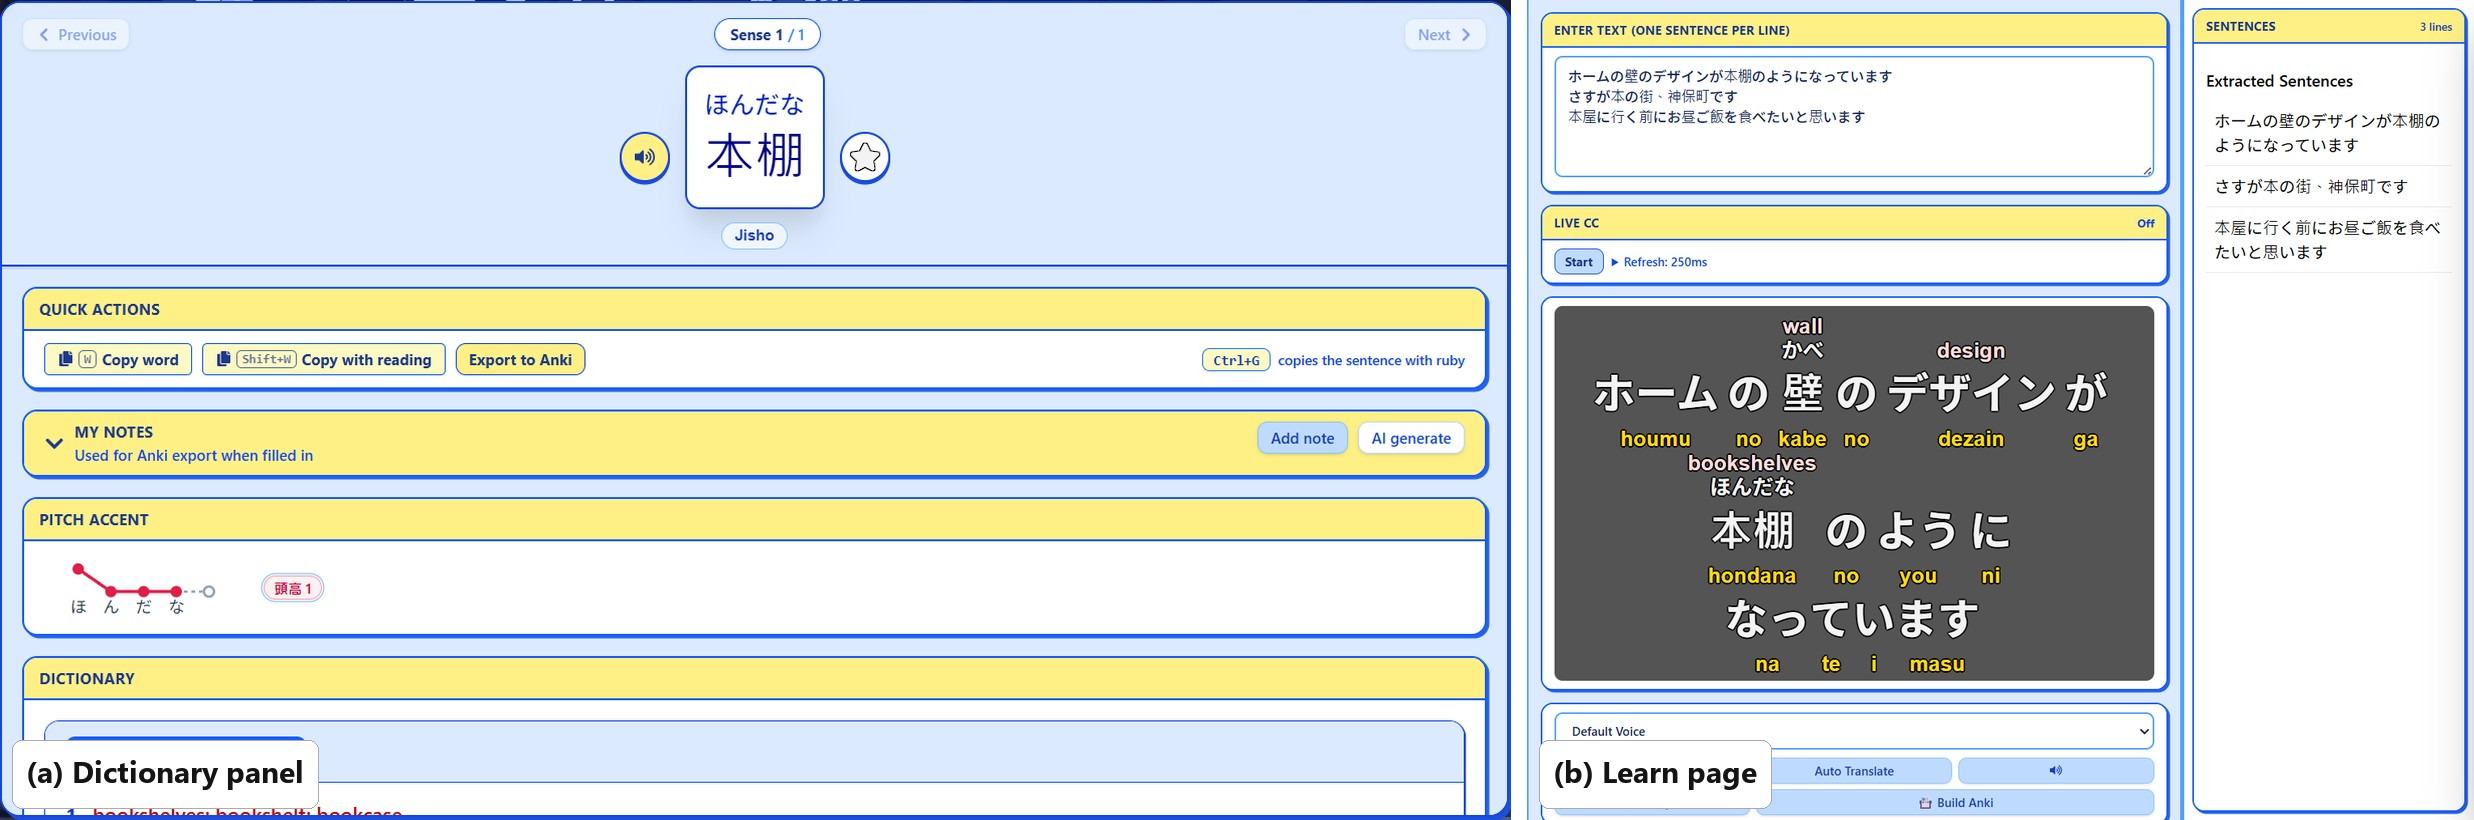
\includegraphics[width=\linewidth]{figures/fig_lookup.jpg}
  \caption{(a) Clicking \emph{hondana} ``bookshelf'' in the Japanese line of Figure~\ref{fig:teaser}: JMdict senses, the reading, and an OJAD-style pitch-accent contour (\emph{atamadaka}, accent on the first mora) from Kanjium data. (b) The Learn page's analyzer and sentence list: pasted sentences are segmented and rendered like subtitles, with glosses above in this layout. The verb phrase \emph{natte imasu} is one merged token.}
  \label{fig:lookup}
\end{figure}

\section{Architecture}
\label{sec:arch}

Miteiru is an Electron application \citep{electron} built with Nextron \citep{nextron}: a Node.js main process and a React renderer compiled as a static Next.js export (Figure~\ref{fig:arch}). It ships for Windows, macOS and Ubuntu, and is licensed CC BY-NC-SA 4.0.

\begin{figure}[t]
\centering
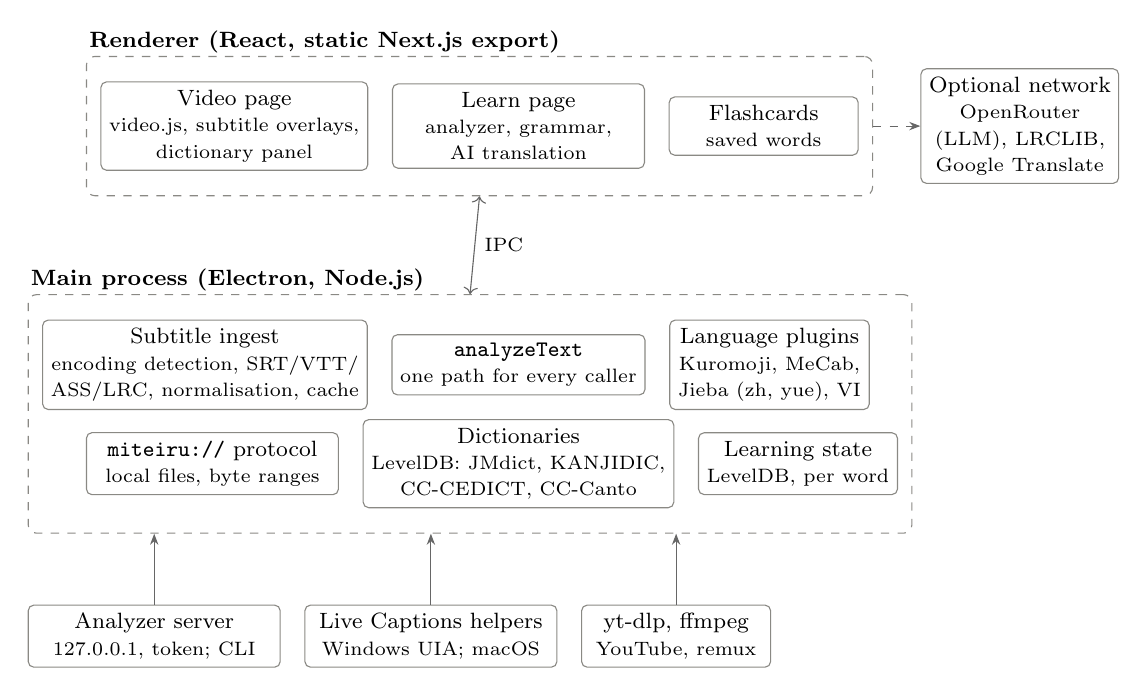
\begin{tikzpicture}[
  font=\footnotesize,
  box/.style={draw=boxline, rounded corners=2pt, align=center, inner sep=3pt, fill=white},
  grp/.style={draw=boxline, dashed, rounded corners=3pt, inner sep=5pt},
  lbl/.style={font=\footnotesize\bfseries, anchor=south west, inner sep=1pt},
  arr/.style={-{Stealth[length=4pt]}, draw=black!60},
]
% renderer
\node[box, minimum width=3.2cm] (video) {Video page\\\scriptsize video.js, subtitle overlays,\\\scriptsize dictionary panel};
\node[box, minimum width=3.2cm, right=3mm of video] (learn) {Learn page\\\scriptsize analyzer, grammar,\\\scriptsize AI translation};
\node[box, minimum width=2.4cm, right=3mm of learn] (flash) {Flashcards\\\scriptsize saved words};
\node[grp, fit=(video)(learn)(flash), inner ysep=9pt] (rend) {};
\node[lbl] at (rend.north west) {Renderer (React, static Next.js export)};

% main process
\node[box, below=21mm of learn, minimum width=3.2cm] (an) {\texttt{analyzeText}\\\scriptsize one path for every caller};
\node[box, left=3mm of an, minimum width=3.2cm] (sub) {Subtitle ingest\\\scriptsize encoding detection, SRT/VTT/\\\scriptsize ASS/LRC, normalisation, cache};
\node[box, right=3mm of an, minimum width=2.4cm] (plug) {Language plugins\\\scriptsize Kuromoji, MeCab,\\\scriptsize Jieba (zh, yue), VI};
\node[box, below=3mm of an, minimum width=3.2cm] (dict) {Dictionaries\\\scriptsize LevelDB: JMdict, KANJIDIC,\\\scriptsize CC-CEDICT, CC-Canto};
\node[box, left=3mm of dict, minimum width=3.2cm] (proto) {\texttt{miteiru://} protocol\\\scriptsize local files, byte ranges};
\node[box, right=3mm of dict, minimum width=2.4cm] (learnst) {Learning state\\\scriptsize LevelDB, per word};
\node[grp, fit=(sub)(an)(plug)(dict)(proto)(learnst), inner ysep=9pt] (main) {};
\node[lbl] at (main.north west) {Main process (Electron, Node.js)};

\draw[arr, <->] (rend.south) -- node[right, font=\scriptsize] {IPC} (main.north);

% external
\node[box, below=9mm of main.south west, anchor=north west, minimum width=3.2cm] (srv) {Analyzer server\\\scriptsize 127.0.0.1, token; CLI};
\node[box, right=3mm of srv, minimum width=3.2cm] (lc) {Live Captions helpers\\\scriptsize Windows UIA; macOS};
\node[box, right=3mm of lc, minimum width=2.4cm] (tools) {yt-dlp, ffmpeg\\\scriptsize YouTube, remux};
\draw[arr] (srv.north) -- (srv.north |- main.south);
\draw[arr] (lc.north) -- (lc.north |- main.south);
\draw[arr] (tools.north) -- (tools.north |- main.south);

\node[box, right=6mm of rend.east, anchor=west, text width=2.3cm, minimum height=1.1cm] (net) {Optional network\\\scriptsize OpenRouter (LLM), LRCLIB, Google Translate};
\draw[arr, dashed] (rend.east) -- (net.west);
\end{tikzpicture}
\caption{Miteiru's architecture. Every tokenization, from subtitle lines, the Learn page, live captions or the local analyzer server, goes through one function in the main process. Network services are optional; the subtitle pipeline runs offline.}
\label{fig:arch}
\end{figure}

\paragraph{One analysis path.}
All tokenization runs in the main process behind a single function, \texttt{analyzeText}, which dispatches on the active language. The renderer calls it over IPC for each subtitle line; the Learn page calls it for pasted text; and a local HTTP server exposes it to other programs. The server binds to 127.0.0.1 on a port chosen by the operating system, requires a random token written to a registration file in the user's data directory, and offers \texttt{/health}, \texttt{/analyze} and \texttt{/analyze-batch}. It cannot switch the language: a request that names a different language gets an error, so outside tools always see exactly what the window shows. The token data in Sections~\ref{sec:languages} and~\ref{sec:cantonese} were collected through this server.

\paragraph{Language plugins and assets.}
Each language is a plugin with dependencies: the Japanese, Mandarin and Cantonese plugins depend on a shared Han-character pack (KanjiVG and Make Me a Hanzi stroke data, WaniKani radicals). Plugins ship as asset packs bundled into the installer; on first use, each JSON dictionary is converted into a LevelDB database in the user's data directory, so later lookups are prefix range scans on disk rather than searches in memory.

\paragraph{Subtitles.}
Subtitle files are decoded after detecting their encoding, which matters for the Shift-JIS, GBK and Big5 files common among older Asian subtitles, then parsed (SRT, VTT, ASS, LRC, and a JSON lyrics format). By default each file is first normalised: lines are sentence-cased, a step meant for all-caps English subtitles, and bracketed sound descriptions and speaker labels are removed. Each line ends 240\,ms late and never overlaps the next, and the current line is found by binary search on start time.

\paragraph{Local media.}
Local video reaches Chromium through a custom \texttt{miteiru://} protocol that serves files with HTTP byte ranges, so seeking works on large files. Files Chromium cannot decode (HEVC, or several audio tracks) are probed with ffprobe and offered a remux or re-encode with ffmpeg; embedded subtitle tracks are extracted the same way.

\paragraph{Live Captions.}
Rather than bundle a speech recogniser, Miteiru reuses the operating system's. On Windows~11, a small .NET helper starts the built-in Live Captions app and reads its caption text through UI Automation every 80\,ms; on Apple Silicon Macs running macOS~26, an Objective-C helper calls the system's private live-transcription framework with the locale of the active language. Both helpers page the rolling transcript into subtitle-sized windows of at most 70 characters and print one JSON object per line, which the main process feeds into the ordinary subtitle path.

\section{Four languages, four pipelines}
\label{sec:languages}

The four languages differ in every respect that matters to a subtitle reader (Table~\ref{tab:languages}): whether words are written with spaces, whether the script shows pronunciation, and what a reading aid has to show. Figure~\ref{fig:tokens} shows each pipeline's output on a real subtitle line.

\begin{table}[t]
\centering
\small
\caption{The four language stacks in Miteiru 7.5.2. Dictionary sizes are the bundled files' entry counts.}
\label{tab:languages}
\begin{tabularx}{\linewidth}{@{}P{2.25cm}YYYY@{}}
\toprule
 & Japanese & Mandarin & Cantonese & Vietnamese \\
\midrule
Script & kanji + kana & Han (Simplified or Traditional) & Han (Traditional, with Cantonese-only characters) & Latin with diacritics \\
Word boundaries & none & none & none & spaces between syllables, not words \\
Reading shown & furigana (hiragana), romaji & pinyin, 4 tones + neutral & Jyutping, 6 tones & none; gloss in its place \\
Segmenter & Kuromoji \citep{kuromojijs}, or MeCab \citep{kudo2004applying} & Jieba \citep{jieba,jiebars}, Mandarin dictionary & Jieba, Cantonese dictionary & backward maximum matching \\
Readings from & tokenizer & pinyin-pro \citep{pinyinpro} & to-jyutping \citep{tojyutping} & --- \\
Dictionary & JMdict \citep{breen2004jmdict}, 206,387 entries; KANJIDIC \citep{kanjidic} & CC-CEDICT \citep{ccedict}, 122,431 words & CC-Canto \citep{cccanto} with CantoDict compounds, 95,399 words & VNEDICT \citep{vnedict}, 54,345 headwords \\
Extras & lemma lookup, conjugation tables, pitch accent (9,255 words, Kanjium \citep{kanjium}), 831 JLPT grammar points & Traditional to Simplified conversion & characters kept as written & --- \\
\bottomrule
\end{tabularx}
\end{table}

\begin{figure}[t]
  \centering
  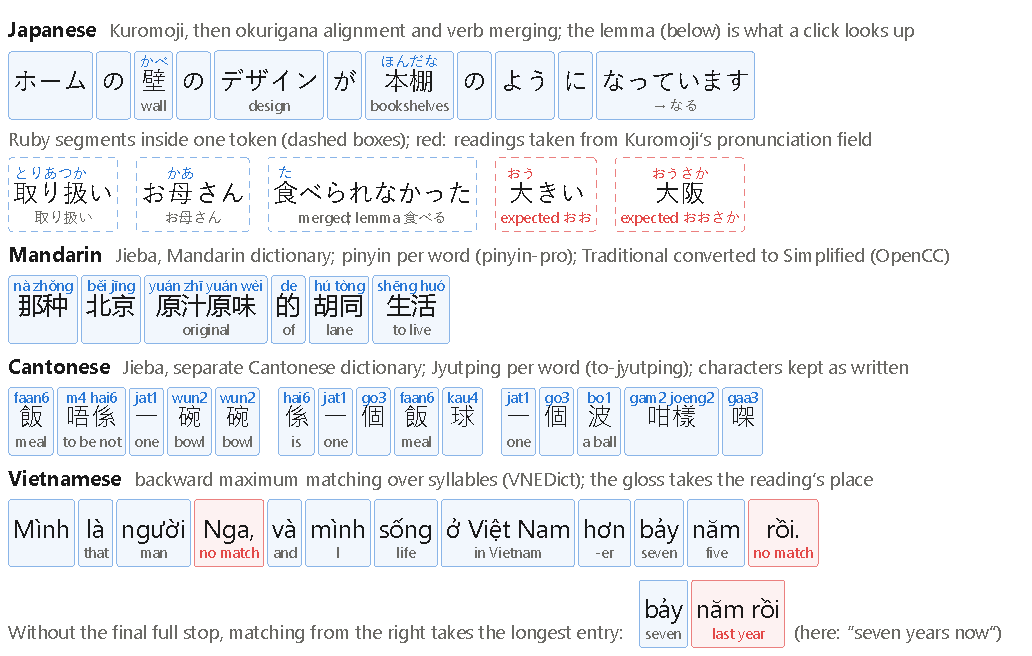
\includegraphics[width=\linewidth]{figures/fig_tokens.pdf}
  \caption{Miteiru's own output on the subtitle lines of Figure~\ref{fig:teaser}, collected through its analyzer server. Boxes are tokens; small text above is the reading and below is the gloss the overlay shows. Red marks an error. Japanese readings come from Kuromoji's pronunciation field, which writes the long \emph{o} of \emph{ooki} and \emph{Oosaka} as \emph{ou}. The Vietnamese line keeps the punctuation attached to the syllable, and matching from the right picks \emph{\viet{n\u{a}m r\`{\^o}i}} ``last year'' where the speaker means ``seven years now''.}
  \label{fig:tokens}
\end{figure}

\subsection{Japanese}

Japanese is segmented by kuromoji.js \citep{kuromojijs} through a small wrapper, with an IPADIC-style dictionary \citep{ipadic}; MeCab \citep{kudo2004applying,mecab} with any of its dictionaries, UniDic \citep{den2008proper,unidic} among them, is an option. Each token's reading is converted to hiragana and then split over the word in at most three parts: leading kana, a kanji core, and trailing okurigana, each part keeping its own reading. So \emph{toriatsukai} gets one reading over its kanji core and none over its last kana, and \emph{okaasan} gets one only over the kanji for ``mother'' (Figure~\ref{fig:tokens}).

A second pass merges a verb with the auxiliaries and particles that follow it, using a deconjugator to check that the merged form still reduces to the verb's dictionary form. \emph{Taberarenakatta} ``could not eat'' becomes one token whose lemma is \emph{taberu}. Because learning state and frequency are counted by lemma, every form of a verb shares one state, and clicking any form opens the dictionary entry. The dictionary panel adds a conjugation table generated from the lemma, with a ``when to use'' note per form, and a pitch-accent contour in the Tokyo pattern that the NHK accent dictionary records \citep{nhk2016accent}, drawn from Kanjium's data \citep{kanjium}. Pitch accent is rarely taught, but training improves learners' identification of it \citep{shport2016training}, and even advanced learners' perception of it depends on their vocabulary \citep{goss2019lexical}, which is an argument for showing it word by word.

The readings have one systematic error. Kuromoji's pronunciation field writes a long vowel with a length mark, and converting that mark to hiragana after an \emph{o}-row kana gives \emph{u}: \emph{ookii} ``big'' is shown as \emph{oukii}, \emph{toori} ``street'' as \emph{touri}, and \emph{Oosaka} as \emph{Ousaka} (Figure~\ref{fig:tokens}). For most words the two spellings sound alike, since \emph{ou} is also pronounced as a long \emph{o}, but the furigana is misspelt, and the same reading feeds the pitch-accent lookup, which then misses those words. Using the dictionary reading for furigana, and keeping the pronunciation for romaji (where the particle \emph{ha} should read \emph{wa}), would fix it.

\subsection{Mandarin}

Mandarin is segmented by Jieba \citep{jieba}, through a Rust port \citep{jiebars}, with a dictionary of about 584,000 words that holds both simplified and traditional forms. Pinyin comes from pinyin-pro \citep{pinyinpro}, called once per word, so polyphonic characters are resolved by the word they are in. Traditional subtitles are converted to simplified by default (a setting reverses it), since most learners' dictionaries and textbooks are simplified.

Tones can be shown two ways (Figure~\ref{fig:tones}). The default replaces the tone number with a small contour glyph and the number, a level bar for tone~1, a rising stroke for tone~2, a dip for tone~3 and a falling stroke for tone~4; the alternative is standard pinyin with diacritics. Miteiru used contour marks for Jyutping first and extended them to Mandarin in August 2026; they draw each tone's pitch shape beside the syllable rather than over a vowel.

\begin{figure}[t]
  \centering
  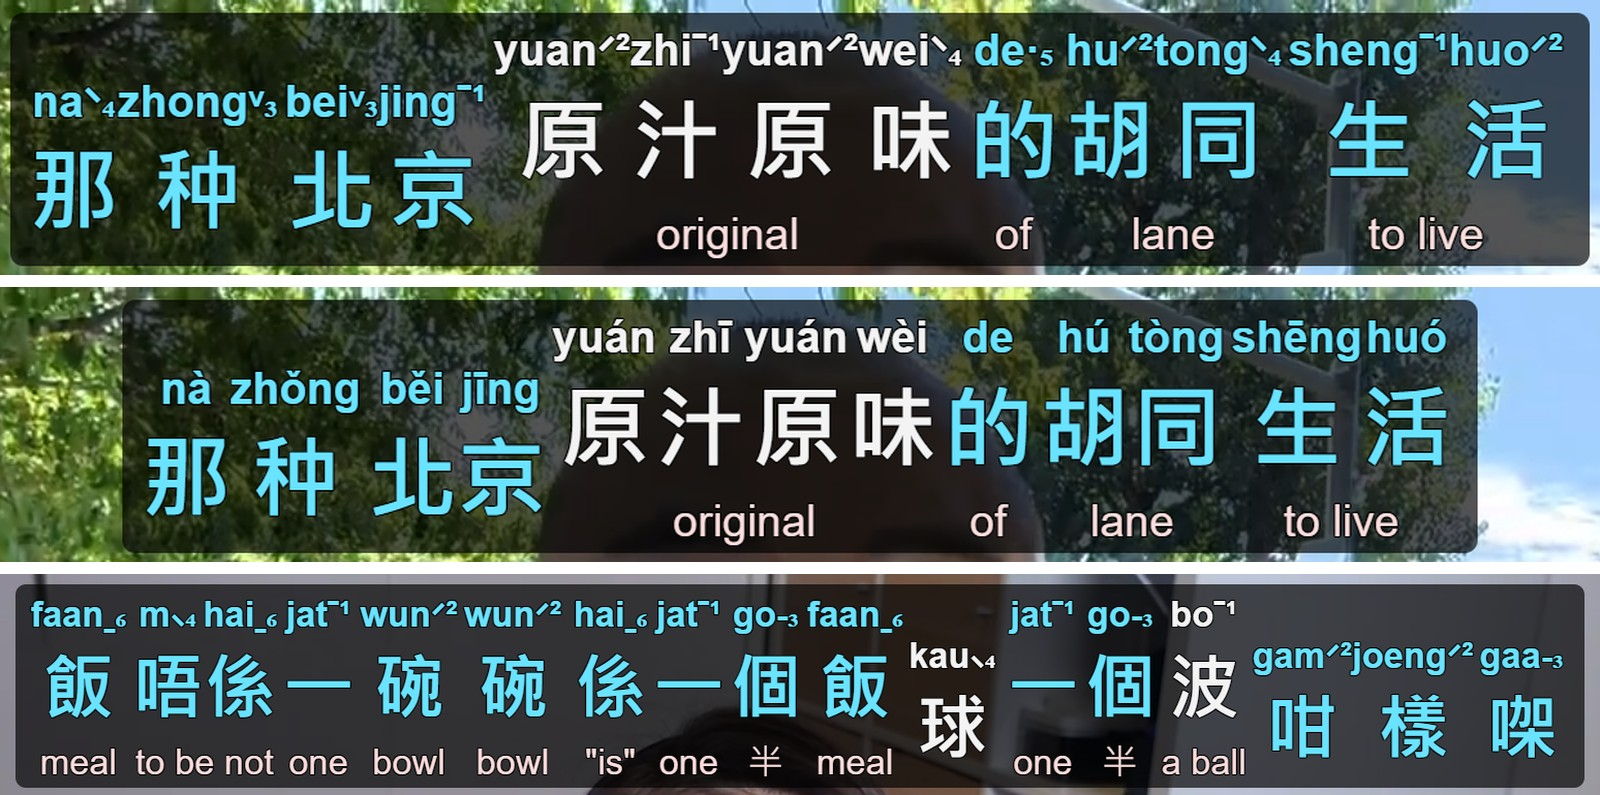
\includegraphics[width=0.92\linewidth]{figures/fig_tones.jpg}
  \caption{Tone display. Top: Mandarin with contour marks (the default). Middle: the same line with standard pinyin diacritics. Bottom: Cantonese Jyutping with contour marks for its six tones.}
  \label{fig:tones}
\end{figure}

\subsection{Vietnamese}
\label{sec:vietnamese}

Vietnamese has the opposite problem from Chinese and Japanese: spaces are everywhere, but they separate syllables, not words, and about 85\% of word types have two or more syllables \citep{nguyen2018fast}. Research segmenters use trained models \citep{nguyen2018fast,vu2018vncorenlp}; Miteiru uses backward maximum matching over syllables against VNEDICT \citep{vnedict}, taking from the right end the longest run of syllables that is a dictionary headword. The written form already tells the learner how to pronounce a word, so the reading slot above the word holds its gloss instead.

The method finds most compounds, \emph{\viet{\h{\ohorn} Vi\d{\^e}t Nam}} ``in Vietnam'' among them, and fails in three measured ways (Figure~\ref{fig:tokens}). Lookup is case-sensitive and punctuation stays attached to the syllable, so a comma or full stop hides the word. Greedy matching takes the longest entry even when the sentence means something else: \emph{\viet{b\h{a}y n\u{a}m r\`{\^o}i}} ``seven years now'' becomes \emph{\viet{b\h{a}y}} plus \emph{\viet{n\u{a}m r\`{\^o}i}} ``last year''. And the default normalisation, meant for all-caps English subtitles, lowercases every line, which turns \emph{\viet{Vi\d{\^e}t Nam}} into two separate dictionary misses; this is visible in Figure~\ref{fig:teaser}, where \emph{nam} is glossed ``male''. The shortest-sense gloss shows the cost of having no context: \emph{\viet{n\u{a}m}} is glossed ``five'' because the dictionary lists ``five'' before ``year''.

\subsection{Display and learning state}
\label{sec:display}

Every language renders through the same component. A token is a nested ruby: the reading above the word, romaji below it for Japanese, and the gloss below or above the whole. Chromium left-aligns ruby annotations under some conditions, so Miteiru lays each ruby out with flexbox to centre the reading; and because \texttt{-webkit-text-stroke} breaks CJK ruby on Windows, the subtitle outline is drawn with eight to twenty-four text shadows instead.

Each word has a learning state: new, learning or known, cycled by right-click and stored per language and word. A fourth state is inferred: words that are among the most frequent in the current subtitle file (by default the top 30\% of word types that occur more than once) and that the learner has not rated are coloured as frequent, so the words worth learning first stand out. For Chinese and Vietnamese the display follows the expertise-reversal result \citep{lee2011onscreen}: a word marked known loses its reading, and new and frequent words always show their gloss. Japanese words change colour only; their furigana does not fade.

\paragraph{Speed.}
Tokenizing a whole subtitle file through the analyzer server, readings included but per-word glosses not, took a median of 53, 44, 44 and 43\,ms for the Japanese, Mandarin, Cantonese and Vietnamese files of Figure~\ref{fig:teaser} (211, 411, 356 and 426 lines; five runs each, Intel Core Ultra~7 265K). Loading a subtitle file is therefore dominated by the per-word dictionary queries for glosses, which run one by one and which this paper did not time.

\section{Why Cantonese is its own language here}
\label{sec:cantonese}

Miteiru's Cantonese mode came before its Mandarin mode, and it was never a setting of it. The reasons are linguistic, orthographic and social.

\paragraph{A different spoken language.}
Cantonese and Mandarin are not mutually intelligible in speech. Cantonese has six tones to Mandarin's four, different finals and initials, and its own grammar and core vocabulary \citep{matthews2011cantonese}: its possessive particle, perfective marker, third-person pronoun, locative verb, negators and copula are different words, not different pronunciations of the Mandarin ones (Figure~\ref{fig:cantonese}). It has its own romanisation, Jyutping \citep{lshkjyutping}, its own corpora and tools \citep{luke2015hkcancor,lee2022pycantonese}, and its own dictionaries, though for language technology it remains under-resourced, colloquial and code-switched \citep{xiang2025cantonese}; Miteiru uses CC-Canto \citep{cccanto} with compounds from CantoDict, and a segmentation dictionary of 35,000 Cantonese words separate from the Mandarin one.

\paragraph{Two ways to write it.}
Cantonese speech can be written in two ways. Standard Written Chinese (SWC) is the written language of Hong Kong schools, newspapers and government; it is grammatically Mandarin, and Cantonese speakers read it aloud in Cantonese pronunciation. Written Cantonese writes down the spoken language, with characters that SWC does not use, and has grown into a vernacular with many, though not all, traits of a standard language \citep{snow2004cantonese,snow2008cantonese}. The two are not spellings of the same sentence. ``We're going to eat roast goose today'' is \emph{ngo5dei6 gam1jat6 heoi3 sik6 siu1ngo2} in speech; its SWC version uses a different pronoun, a different word for ``today'' and a different verb for ``eat'', and read in Cantonese it comes out as \emph{ngo5mun4 gam1tin1 heoi3 hek3 siu1ngo2}, which no one says (Figure~\ref{fig:cantonese}).

\begin{figure}[t]
  \centering
  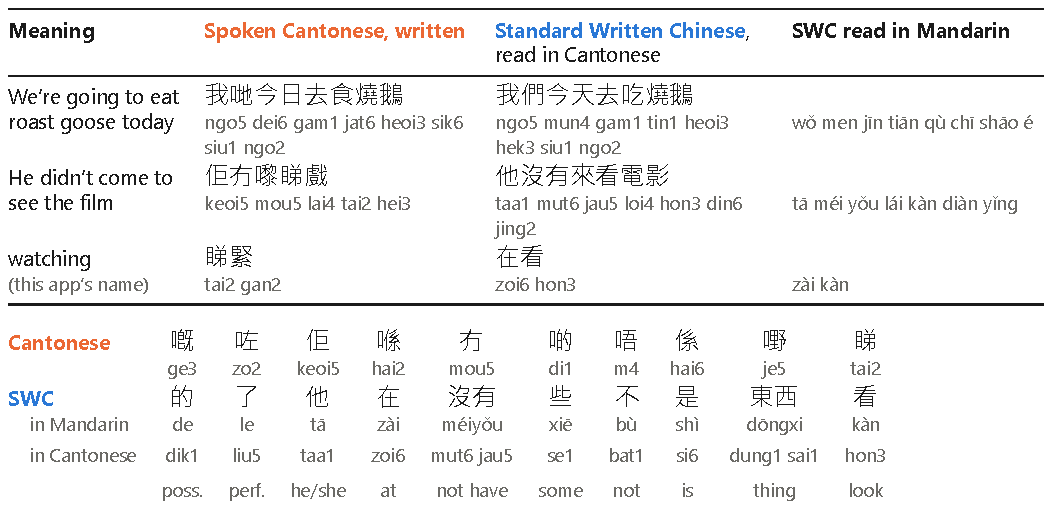
\includegraphics[width=\linewidth]{figures/fig_cantonese.pdf}
  \caption{Spoken Cantonese written down, against Standard Written Chinese (SWC) with the same meaning, as Miteiru reads them. Top: whole sentences, including the app's own name, ``watching''. Bottom: ten function and core words whose Cantonese form is a different word from SWC's. Jyutping and pinyin are Miteiru's output through its analyzer server, except the particle readings of the SWC perfective (\emph{le}) and possessive (\emph{de}), which it gives in isolation as \emph{liao3} and \emph{de}.}
  \label{fig:cantonese}
\end{figure}

\paragraph{Subtitles are usually SWC.}
Hong Kong subtitling is diglossic: SWC is the norm for subtitles, and written Cantonese appears for low-register speech such as swearing \citep{yau2012power,chen2004hong}. To see what a learner meets on YouTube today, I screened videos found by five Cantonese-language searches (vlogs, cooking, street interviews) filtered to videos with subtitles. Of 37 videos, 27 had an uploader-made subtitle track in a Chinese language code; I downloaded the 24 under 30 minutes long and counted, in each, 26 characters that mark written Cantonese (the forms in Figure~\ref{fig:cantonese} and sentence particles) against 15 SWC forms (their counterparts and common function words). The score is the Cantonese share of all marker hits.

\begin{table}[t]
\centering
\small
\caption{Register of uploader-made Chinese subtitles on 22 YouTube videos found by Cantonese searches (two of the 24 downloaded tracks had no marker hits). The scores are bimodal: a subtitler writes one register or the other.}
\label{tab:register}
\begin{tabular}{@{}lrrr@{}}
\toprule
Register (Cantonese share of marker hits) & Videos & Channels & Marker hits, median \\
\midrule
Standard Written Chinese ($\le$\,0.03) & 15 & 14 & 189 \\
Mixed (0.28) & 1 & 1 & 72 \\
Written Cantonese ($\ge$\,0.95) & 6 & 3 & 266 \\
\bottomrule
\end{tabular}
\end{table}

Fifteen of the 22 tracks were SWC and six were written Cantonese, four of those from one channel (Table~\ref{tab:register}); only one mixed the two. A full-time Cantonese teacher's vlog, among others, was subtitled in SWC (3 Cantonese markers against 152 SWC ones). The screen is small and its searches are not a sample of YouTube, and I did not verify the spoken language of every video; it shows only that SWC subtitles over Cantonese speech are common enough that a Cantonese mode must expect them.

\paragraph{What this means for a learner, and for Miteiru.}
With SWC subtitles, a learner of Cantonese reads one sentence and hears another. Miteiru's Cantonese mode segments and reads whatever is written, so on an SWC line it shows the literary reading of each SWC word, \emph{taa1} for ``he'' where the speaker says \emph{keoi5}. That is correct as a reading of the text and wrong as a guide to the audio. Miteiru handles it in three ways today: it keeps Cantonese apart, so Cantonese-only characters, Jyutping and Cantonese compounds are always available; it keeps characters as written instead of converting them, as the Mandarin mode does; and its AI translation is told to write ``written Cantonese in Traditional Chinese'' and to prefer distinctly Cantonese wording over SWC, so a learner can produce the spoken form. Aligning an SWC subtitle with what was actually said, for example by showing a Cantonese live caption beside it, is open (Section~\ref{sec:future}).

\section{Design decisions}
\label{sec:decisions}

Table~\ref{tab:decisions} lists twelve decisions that shaped Miteiru. Each was checked against the repository: the date is the commit, release or issue where the decision shows.

\begin{table}[p]
\centering
\small
\caption{Design decisions, the alternative each rejected, and where the history shows them. Era: \textcolor{preai}{\textbf{P}} pre-AI (before September 2025), \textcolor{withai}{\textbf{A}} AI-assisted.}
\label{tab:decisions}
\renewcommand{\arraystretch}{1.18}
\begin{tabularx}{\linewidth}{@{}p{0.3cm}P{3.1cm}P{2.6cm}YP{2.2cm}@{}}
\toprule
 & Decision & Instead of & Why & Evidence \\
\midrule
\textcolor{preai}{\textbf{P}} & A desktop player for local files & a browser extension over streaming sites & learners' subtitles are files (ASS fansubs, SRT, LRC); offline; any codec Chromium plays & first commits, Dec 2022 \\
\textcolor{preai}{\textbf{P}} & Kuromoji built in, MeCab optional & requiring a MeCab install & MeCab had to be installed and located by hand; the issue asks for ``better UX'' & issue 32, PR 35, Jul 2023 \\
\textcolor{preai}{\textbf{P}} & Dictionaries bundled, cached in LevelDB & an online dictionary API & offline, private, fast prefix lookup & asset release, Aug 2023 \\
\textcolor{preai}{\textbf{P}} & Cantonese as its own language & a Mandarin setting & separate words, readings, dictionary and segmentation (Section~\ref{sec:cantonese}) & Cantonese mode 19 Dec 2023; Mandarin 15 Jan 2024 \\
\textcolor{preai}{\textbf{P}} & Readings above every word, glosses below & a separate dictionary pane only & readings above the character beat readings beside it \citep{lee2011effectiveness} & first releases \\
\textcolor{preai}{\textbf{P}} & Learning state by colour; readings fade for known Chinese words & always-on readings & expertise reversal \citep{lee2011onscreen}; frequent words stand out & learning state, Feb 2024 (issue 57) \\
\textcolor{preai}{\textbf{P}} & Export to Anki; drop the in-app spaced repetition & building an SRS & Anki already schedules well \citep{settles2016trainable}; the in-app SRS was removed as a ``gimmick'' & SRS Jun 2024 (issue 59), removed May 2025 \\
\textcolor{withai}{\textbf{A}} & Deterministic pipeline; LLMs optional and outside it & LLM tokenization or readings & offline, reproducible, free; an LLM never decides a reading in the subtitle path & AI features from Dec 2025 \\
\textcolor{withai}{\textbf{A}} & LLM output constrained by symbolic tools & free-form generation & example sentences must use a conjugated form from the table; ruby HTML is built locally from the LLM's segments & v6.5.0, v7.4.3, Jul 2026 \\
\textcolor{withai}{\textbf{A}} & Reuse the operating system's speech recognition & bundling an ASR model & no model download; same overlay for any audio; cost: undocumented interfaces & v6.0.0 Apr 2026; v7.5.1 Aug 2026 \\
\textcolor{withai}{\textbf{A}} & One analysis path, exposed on localhost & a separate API implementation & tools see what the window shows; the API cannot switch language & v6.1.0, Jun 2026 \\
\textcolor{withai}{\textbf{A}} & Deterministic Anki note IDs & new notes on each export & re-importing updates notes instead of duplicating them & v6.2.0, Jul 2026 \\
\bottomrule
\end{tabularx}
\end{table}

Three of them need more than a table row.

\paragraph{Offline first, AI optional.}
Miteiru's core was designed before large language models were practical for this job, and it stayed deterministic after they were. Segmentation, readings, glosses and dictionary lookup use tokenizers and dictionaries; an LLM is called only when the learner asks for a translation, an analysis, notes, example sentences or an Anki card, and only with the learner's own API key. Where an LLM's output meets the rest of the system, a symbolic tool bounds it: conjugation examples are accepted only for the exact forms the conjugation library produced, and when an LLM segments a sentence for an Anki card, Miteiru escapes the text and builds the ruby markup itself rather than accepting HTML from the model.

\paragraph{Anki instead of an SRS.}
Miteiru had its own spaced-repetition page from June 2024 until May 2025, when it was removed. Spaced repetition works \citep{cepeda2006distributed}, and good schedulers exist \citep{settles2016trainable,anki}; building another one did not help learners who already used Anki. Miteiru instead writes Anki's import format with deterministic note IDs, derived from the language and the normalised word, so exporting the same word again updates its note. A simple flashcards page remains for reviewing saved words in the app.

\paragraph{Borrowing the OS's ears.}
Live Captions reuse the speech recogniser the operating system already has, which costs no download and covers whatever audio is playing, including streams and calls. The cost is that both integrations rest on interfaces Microsoft and Apple do not document for this use: reading another app's window through accessibility APIs on Windows, and a private framework on macOS. Either can break with an operating-system update.

\section{Building it before and with AI coding assistants}
\label{sec:history}

Miteiru's first commit came weeks after ChatGPT's public release, but for its first 32 months it was written without AI coding assistants. The author began using them in September 2025, mainly Cursor \citep{cursor}. The history is therefore a natural record of one developer's project across the change. This section compares the two eras.

\paragraph{Data.}
The analysis uses the 633 commits on the first-parent history of the main branch, from 18 December 2022 to 2 September 2026 (737 commits including merged branches). For each commit it counts changed lines in hand-written files, excluding the lock file, generated and bundled data, and images; code size is the line count of source files (TypeScript, JavaScript, Python, C\#, Objective-C, CSS) at the end of each month. The era boundary is 1 September 2025, from the author's account. The repository itself first shows AI involvement later: the first commit with a Cursor co-author trailer is dated 13 June 2026 and the first Cursor configuration file 11 July 2026, and only 36 commits carry the trailer. Trailers undercount agent commits \citep{khosravani2026detecting}, so the boundary rests on the author's account, with the repository's traces as a lower bound.

\begin{figure}[t]
  \centering
  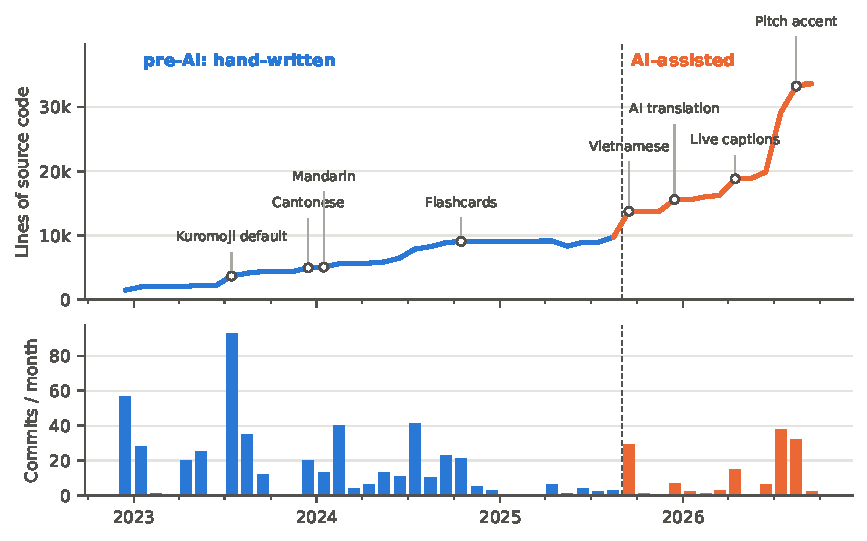
\includegraphics[width=\linewidth]{figures/fig_history.pdf}
  \caption{Code size at the end of each month (top) and commits per month (bottom), pre-AI in blue and AI-assisted in orange. The dashed line is September 2025. Labels mark when each language and some major features arrived.}
  \label{fig:history}
\end{figure}

\begin{table}[t]
\centering
\small
\caption{The two eras. Changed lines exclude the lock file, generated data and images.}
\label{tab:eras}
\begin{tabular}{@{}lrr@{}}
\toprule
 & \textcolor{preai}{\textbf{Pre-AI}} & \textcolor{withai}{\textbf{AI-assisted}} \\
 & Dec 2022 -- Aug 2025 & Sep 2025 -- Sep 2026 \\
\midrule
Span (days) & 959 & 364 \\
Commits & 497 & 136 \\
Days with a commit & 105 & 38 \\
Commits per active day & 4.7 & 3.6 \\
Lines changed per commit (median / mean / p90) & 13 / 57 / 156 & 89 / 308 / 970 \\
Code lines added / deleted & 19,003 / 9,296 & 32,880 / 9,059 \\
Source lines at the era's end & 9,711 & 33,600 \\
Test files at the era's end & 0 & 33 \\
Commit subject, median words & 3 & 4 \\
Commits with a message body & 3\% & 33\% \\
Commits with a Cursor co-author trailer & 0 & 36 \\
Releases / release downloads & 40 / 2,877 & 16 / 1,106 \\
\bottomrule
\end{tabular}
\end{table}

\paragraph{What changed.}
The AI-assisted era wrote more code in less time (Table~\ref{tab:eras}, Figure~\ref{fig:history}). In 12 months the code grew from 9.7k to 33.6k source lines, 3.5 times its size after 32 months of hand-written work. The commits became bigger rather than more frequent: the median commit changed 89 lines instead of 13, and the 90th percentile 970 instead of 156. The project also gained what it never had: a test suite (33 test files, 260 test cases, run in continuous integration), release notes for every version from 6.0.0, a JSON schema for its dictionaries, and escaping where dictionary and LLM text becomes HTML. Commit messages changed from terse labels (``Add video page'', ``Update package'') to sentences with bodies: in August 2026 the median subject was nine words.

The feature mix changed too (Figure~\ref{fig:history}). The pre-AI era built the core a learner touches every minute: the player, Japanese segmentation and readings, the dictionary panel, verb merging, kanji pages, YouTube support, Cantonese and Mandarin, learning states and karaoke. The AI-assisted era added breadth around it: Vietnamese, Live Captions on two operating systems, the analyzer server, AI translation and notes, JLPT grammar study, conjugation tables, pitch accent, Anki decks for notes, sentences and grammar, and LRCLIB lyrics.

\paragraph{What the history cannot show.}
The comparison confounds AI assistance with everything else that changed. Activity had nearly stopped in the eight months before September 2025 (16 commits from January to August 2025), so the second era also measures renewed attention. Lines of code measure size, not value, and larger commits are partly a change of habit. The code written in the second era has not had time to show its maintenance cost, which is where the strongest evidence on these tools points \citep{he2026speed,liu2026debt}. Several bugs found while preparing this paper sit in code from both eras (Section~\ref{sec:limitations}). What the record does show is a single developer's project whose second year with AI assistance produced more than its first three without, while its core design decisions were made before.

\section{Deployment}
\label{sec:deployment}

Miteiru has no telemetry, so its use can be seen only on GitHub. As of 8 October 2026 the repository had 117 stars (1 given in 2022, 31 in 2023, 52 in 2024, 23 in 2025, 10 in 2026), 4 forks and 7 watchers. Its 56 application releases had been downloaded 3,983 times: 1,933 Windows, 1,543 Linux and 347 macOS assets, plus 160 other files; the separate language-asset release had 586 downloads. Release assets have been replaced over the years, so these are lower bounds. Releases from the pre-AI era account for 2,877 downloads and those from the AI-assisted era for 1,106; the later releases have had less time.

The issue tracker served mostly as the author's own backlog: of 52 issues, 43 were opened by the author. Six other people opened the remaining nine, about build failures on Linux and Windows, YouTube subtitles, MKV playback, and Cantonese segmentation and dictionary sources, and one of them contributed a pull request that improved YouTube subtitles. The oldest open issue, a request to support Korean, has 13 comments.

\section{Limitations}
\label{sec:limitations}

\paragraph{No learner study.}
This paper describes a system and its history; it does not measure learning. The design follows published results on subtitles and reading aids (Section~\ref{sec:background}), but whether Miteiru's combination of them helps learners, and how much the fading readings help, is untested.

\paragraph{Pipeline errors.}
The errors in Figure~\ref{fig:tokens} are systematic: Japanese long-\emph{o} readings, Vietnamese punctuation, case and greedy matches, and glosses chosen by length rather than context. Japanese merges most verb forms but not all (\emph{itta} ``went'' stayed two tokens). Glosses take the shortest dictionary sense, which is often not the sense in the sentence.

\paragraph{Defaults that remove text.}
Two subtitle normalisations are on by default and were designed for English subtitles. Sentence-casing lowercases every line, not only all-caps ones, which breaks Vietnamese lookups. Removing hearing-impaired annotations deletes text inside brackets, including the corner brackets that Japanese subtitles use for quoted speech.

\paragraph{Smaller defects found while preparing this paper.}
Running the released build on a fresh profile showed that the secondary track's default style is the primary track's, so translations overlap the primary line until the style is reset; conjugation tables list bare stems as separate forms; a dictionary entry with no senses is shown as an empty list rather than as missing; and the MeCab path chosen in the interface is not passed to the tokenizer. None of them affects the measurements above.

\paragraph{The author is the designer, user and analyst.}
The account of why decisions were made is the author's, checked against the repository but not independent of it \citep{desjardins2018revealing}. The era boundary is the author's account; the repository's own traces start later.

\section{Future work}
\label{sec:future}

The most useful study is the one this paper lacks: learners using Miteiru against a dual-subtitle baseline, in the manner of \citet{kovacs2014smart}, with a condition for fading readings. For Cantonese, the open problem is the gap between SWC subtitles and speech; showing the operating system's Cantonese live caption beside an SWC subtitle, or aligning the two, would let a learner see both. Korean, the longest-standing request, needs a morphological analyser and a reading aid that Hangul does not need for pronunciation but learners may want for Sino-Korean words. And the Japanese and Vietnamese errors above have direct fixes: the dictionary reading instead of the pronunciation field, and punctuation- and case-aware matching.

\section{Conclusion}
\label{sec:conclusion}

Miteiru is an attempt to make every word of real video a lookup, in four languages whose scripts hide pronunciation or word boundaries in different ways. Its main design choices are an offline, deterministic pipeline with AI kept to an optional layer, reading aids above the word that fade as words are learned, and a Cantonese mode that is not a Mandarin setting, because Cantonese video is often subtitled in a written language its speakers do not speak. Its history adds a small, concrete case to the evidence on AI-assisted development: the core design came from two and a half years of hand-written work, and the following year with AI assistance tripled the code and added tests, documentation and breadth. Whether that year's code ages as well as the first is the next thing its history will show.

\section{Availability}
\label{sec:availability}

Miteiru's source and releases are at \url{https://github.com/hockyy/miteiru} \citep{miteiru}. This paper's source, its data (per-commit statistics, monthly code size, the analyzer's token output for every example and its timings, and the Cantonese subtitle screen) and the sources of its diagrams are at \url{https://github.com/hockyy/miteiru-paper}.

\section*{Acknowledgements}
The YouTube creators whose videos appear in Figures~\ref{fig:teaser}--\ref{fig:tones} are credited in Appendix~\ref{app:sources}. The repository survey, measurements, screenshots and draft of this paper were prepared with Claude (Anthropic) under the author's direction; the author checked the claims and is responsible for the content.

\bibliographystyle{plainnat}
\bibliography{refs}

\appendix
\section{Video sources}
\label{app:sources}

The screenshots use frames and subtitle tracks from four public YouTube videos, chosen because their uploaders subtitled the speech in the language spoken, which was checked against YouTube's metadata where it records the speech language. Titles are transliterated.
\begin{itemize}
  \item Japanese: Akane-teki Nihongo Kyoushitsu, ``[Tokyo Vlog] Jinbouchou de ohirugohan o tabete hon'ya ni ikimashita'' (lunch in Jimbocho and a bookshop), 18 September 2025, \url{https://www.youtube.com/watch?v=_e-uQOtIEMY}. Japanese and English tracks.
  \item Mandarin: Da Qi, ``Beijing Caochang hutong you difang 0 youke'' (a Beijing hutong with no tourists), 12 September 2026, \url{https://www.youtube.com/watch?v=y0HlnpFoAHk}. Chinese track.
  \item Cantonese: McFatty Mak Fa Tin, ``Hainan chicken rice (easy rice-cooker version), with Cantonese subtitles, Ep32'', 9 May 2021, \url{https://www.youtube.com/watch?v=E2gaC2a7C3A}. Written-Cantonese track (yue-HK).
  \item Vietnamese: Anh Tay Bao Minh, ``Nguoi Viet tot voi toi den muc toi khong hieu noi'' (Vietnamese people are so kind to me I can't understand it), 6 October 2026, \url{https://www.youtube.com/watch?v=CoUJ406wer0}. Vietnamese track.
\end{itemize}

\end{document}






